\chapter{Evaluation and Analysis}\label{sec:results}

The scripts that perform the evaluation of our testing set, are \texttt{evaluation.sh} and \texttt{exec\_query.sh}.

\section{Video Identification}
After receiving a list of matching windows from the KD-Tree, we classify each one of them as a proper \textbf{match} iff the window's ID matches the ID of the capture we passed to the Java identification process, whereas, if the ID of the capture and the window ID are different, we classify the returned window as a \textbf{mismatch}.

We then report, for various $\omega$ window sizes, the accuracy of our method, to be the proportion of matches with respect to the number of mismatches over the total number of returned windows as:

Let $n$ be the number of returned windows for a given capture trace, and let $TP$ represent the number of matches, and $FP$ to represent the number of returned mismatches:

It follows that $n = TP + FP$

\begin{equation*}
    \mathbf{acc} = \dfrac{TP}{n} = 1 - \dfrac{FP}{n}
\end{equation*}

As mentioned in \Cref{sec:testing}, our testing dataset consists of the same 100 movies present in the database at 8 unseen enforced bandwidths. We pass each capture to the identification process, that runs the evaluation by varying the window size $\omega$, and the corresponding key size $\kappa$. For every run, we then compute the number of matches/mismatches, and report the statistics shown in \Cref{lst:stats}. In addition, we plot for each configuration the number of matches, the number of collisions and the number of mismatches. The number of collisions, represents the number of matches from different bandwidth levels, (e.g. suppose to have a capture at 6.0 \emph{Mbps}, now assume the KDTree returns as matching windows, a list of matches all of the same movie, but at different bandwidths, 5.0 \emph{Mbps}, and 7 \emph{Mbps}, then the number of collisions is 2).

%\begin{figure}[!h]
  %\centering
  %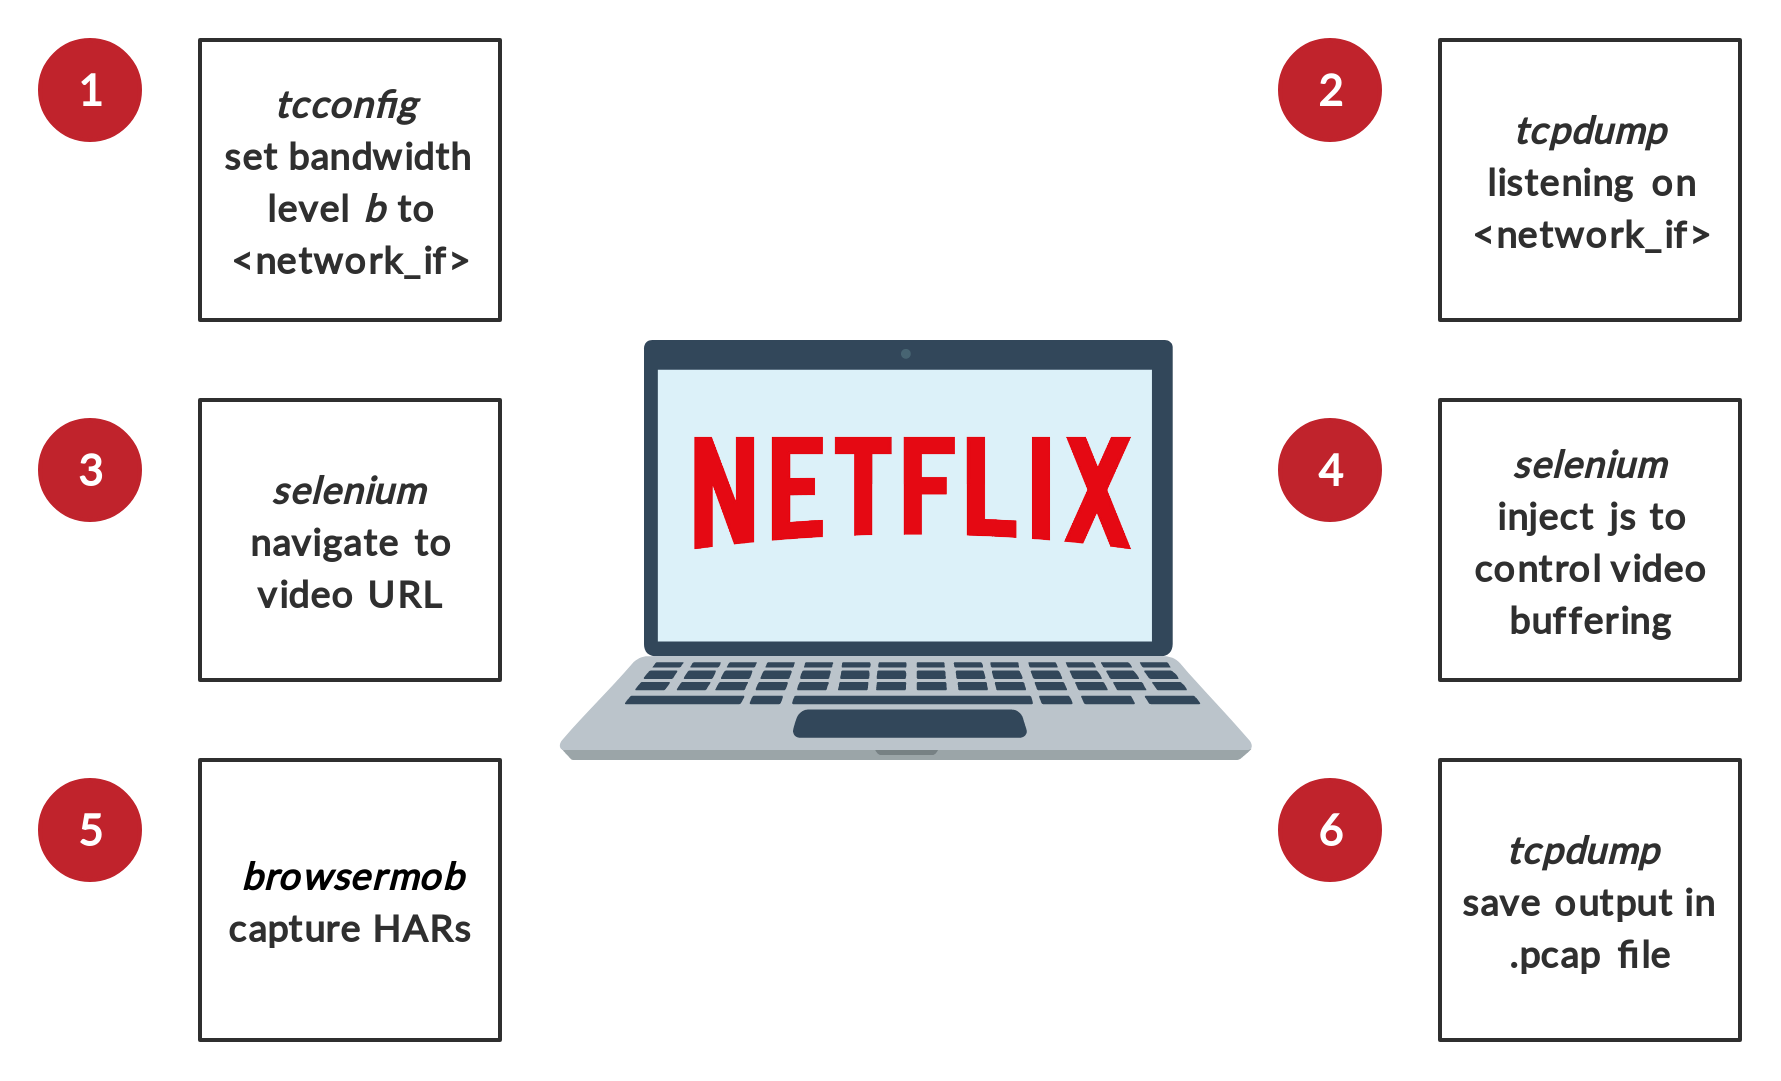
\includegraphics[width=\columnwidth]{img/fingerprints.png}
  %\caption{Overview of the process of acquiring video fingeprints.}
  %\label{fig:fingerprints}
%\end{figure}

\section{Bitrate Ladders}

At first, we evaluate the accuracy of the reconstruced bitrate ladders by computing the RMSE between each one and its corresponding HAR-based bitrate ladder. We have decided to use the RMSE, as it is a well-known indicator that aggregates the residuals to give a measure of the magnitude of error in our predictions, and it is computed as follows.

Let $Y=\{y_1, y_2 \dots y_n\}$ be the set of HAR-based bitrates for movie $m$, at enforced bandwidth
$b$, and let $\hat{Y}=\{\hat{y}_1, \hat{y}_2 \dots \hat{y}_n\}$ be the set of ADU-based computed bitrates for the same
movie at the same enforced bandwidth, then:

\begin{equation*}
    \mathbf{RMSE_{m, b}} = \sqrt{\dfrac{\Sigma_{i=0}^{n}(y_i - \hat{y}_i)^2}{n}}
\end{equation*}

where $n = |Y| = |\hat{Y}|$

Then, the \emph{mean-normalized} RMSE is given by:

\begin{equation*}
    \mathbf{NRMSE_{m, b}} = \dfrac{RMSE_{m, b}}{\overline{\hat{y}}}
\end{equation*}

In addition, in order to assess the uniqueness of both the real and the
reconstrcuted bitrate ladders, we compute, for each bitrate ladder, its average
bitrate, the bitrate standard deviation, and the median.

\begin{small}
\begin{longtable}{|c|c c c|c c c|c|}
    \caption{Collected statistics for the bitrate ladders (values in
    \emph{Mbps})}\label{tab:bitrate_ladders_stats}\\
\hline
\textbf{Title ID} &
\multicolumn{3}{c|}{\textbf{Real}} &
\multicolumn{3}{c|}{\textbf{Reconstruced}} &
\multirow{2}{*}{\textbf{RMSE}} \\
& $\mu$ & $\sigma$ & $\tilde{y}$ & $\mu$ & $\sigma$ & $\tilde{y}$ & \\
\hline
\endhead
\hline
\endfoot
1151721 & 0.77 & 0.25 & 0.92 & 0.73 & 0.27 & 0.88 & 0.09 \\
14607635 & 0.81 & 0.25 & 0.95 & 0.74 & 0.27 & 0.89 & 0.12 \\
328438 & 0.88 & 0.34 & 1.06 & 0.89 & 0.37 & 1.06 & 0.06 \\
60000870 & 1.22 & 0.80 & 1.03 & 1.13 & 0.90 & 0.89 & 0.12 \\
60004481 & 0.75 & 0.19 & 0.85 & 0.65 & 0.19 & 0.76 & 0.16 \\
60020801 & 0.88 & 0.33 & 1.06 & 0.84 & 0.35 & 1.00 & 0.08 \\
60027695 & 0.93 & 0.38 & 1.13 & 0.92 & 0.41 & 1.08 & 0.06 \\
\rowcolor{lightgray}60033314 & 0.45 & 0.03 & 0.46 & 0.30 & 0.06 & 0.34 & 0.50 \\
70019012 & 1.59 & 1.09 & 1.40 & 1.52 & 1.15 & 1.25 & 0.07 \\
70021636 & 0.98 & 0.43 & 1.21 & 0.91 & 0.42 & 1.01 & 0.13 \\
70039177 & 0.66 & 0.16 & 0.74 & 0.58 & 0.21 & 0.66 & 0.18 \\
70041162 & 0.94 & 0.36 & 1.12 & 0.91 & 0.38 & 1.08 & 0.07 \\
70052701 & 1.40 & 1.10 & 1.07 & 1.30 & 1.18 & 0.95 & 0.10 \\
70084788 & 0.77 & 0.26 & 0.89 & 0.74 & 0.30 & 0.87 & 0.09 \\
70102778 & 0.73 & 0.23 & 0.87 & 0.71 & 0.26 & 0.85 & 0.08 \\
70103763 & 1.18 & 0.54 & 1.31 & 1.19 & 0.61 & 1.33 & 0.08 \\
70104894 & 0.82 & 0.28 & 0.96 & 0.78 & 0.31 & 0.92 & 0.09 \\
70112732 & 0.78 & 0.27 & 0.94 & 0.76 & 0.29 & 0.92 & 0.07 \\
70123542 & 0.86 & 0.31 & 1.03 & 0.81 & 0.33 & 0.94 & 0.10 \\
70123920 & 1.06 & 0.46 & 1.33 & 1.03 & 0.47 & 1.25 & 0.08 \\
70130445 & 0.68 & 0.10 & 0.70 & 0.60 & 0.12 & 0.68 & 0.15 \\
70167075 & 0.87 & 0.32 & 1.04 & 0.82 & 0.33 & 1.00 & 0.08 \\
70181730 & 1.80 & 1.65 & 1.51 & 1.75 & 1.59 & 1.44 & 0.09 \\
70208599 & 0.70 & 0.23 & 0.83 & 0.67 & 0.23 & 0.79 & 0.07 \\
\rowcolor{lightgray}70213513 & 0.66 & 0.12 & 0.70 & 0.51 & 0.14 & 0.59 & 0.29 \\
70216224 & 1.06 & 0.45 & 1.34 & 0.93 & 0.45 & 1.14 & 0.18 \\
70220028 & 0.83 & 0.17 & 0.90 & 0.69 & 0.18 & 0.80 & 0.21 \\
70243464 & 1.69 & 1.24 & 1.45 & 1.57 & 1.26 & 1.24 & 0.11 \\
70251894 & 0.79 & 0.25 & 0.93 & 0.76 & 0.30 & 0.92 & 0.10 \\
70264803 & 1.07 & 0.44 & 1.30 & 1.02 & 0.46 & 1.22 & 0.08 \\
70295915 & 0.48 & 0.08 & 0.51 & 0.44 & 0.10 & 0.49 & 0.13 \\
70296965 & 1.43 & 0.83 & 1.48 & 1.40 & 0.87 & 1.33 & 0.10 \\
70297757 & 0.63 & 0.18 & 0.72 & 0.61 & 0.19 & 0.72 & 0.07 \\
\rowcolor{lightgray}70298735 & 0.43 & 0.05 & 0.45 & 0.35 & 0.05 & 0.38 & 0.25 \\
\rowcolor{lightgray}70301367 & 0.44 & 0.05 & 0.46 & 0.33 & 0.07 & 0.36 & 0.35 \\
70305893 & 1.08 & 0.39 & 1.30 & 0.98 & 0.40 & 1.21 & 0.13 \\
70308278 & 1.44 & 1.03 & 1.09 & 1.25 & 1.04 & 0.90 & 0.16 \\
80000643 & 2.44 & 1.41 & 1.99 & 2.37 & 1.41 & 1.94 & 0.05 \\
80009431 & 1.64 & 1.10 & 1.43 & 1.56 & 1.17 & 1.27 & 0.10 \\
80013870 & 1.03 & 0.19 & 1.09 & 0.95 & 0.18 & 1.03 & 0.11 \\
80018689 & 1.05 & 0.44 & 1.24 & 1.00 & 0.46 & 1.16 & 0.08 \\
80023001 & 1.49 & 0.89 & 1.40 & 1.34 & 0.93 & 1.18 & 0.14 \\
80029196 & 1.12 & 0.32 & 1.30 & 0.98 & 0.31 & 1.16 & 0.15 \\
80031611 & 1.39 & 0.73 & 1.37 & 1.26 & 0.77 & 1.26 & 0.13 \\
80031715 & 1.01 & 0.44 & 1.17 & 0.99 & 0.44 & 1.19 & 0.06 \\
80033394 & 0.96 & 0.38 & 1.16 & 0.93 & 0.42 & 1.17 & 0.08 \\
80038359 & 0.84 & 0.31 & 0.99 & 0.82 & 0.32 & 0.96 & 0.06 \\
80052541 & 1.32 & 0.70 & 1.23 & 1.12 & 0.77 & 1.00 & 0.20 \\
80075563 & 1.40 & 0.65 & 1.26 & 1.24 & 0.72 & 1.04 & 0.16 \\
80081155 & 1.70 & 1.22 & 1.39 & 1.71 & 1.37 & 1.27 & 0.11 \\
80081770 & 1.13 & 0.44 & 1.35 & 1.00 & 0.49 & 1.22 & 0.15 \\
80091741 & 1.84 & 1.56 & 1.39 & 1.84 & 1.70 & 1.32 & 0.10 \\
80091879 & 1.08 & 0.48 & 1.34 & 1.02 & 0.49 & 1.28 & 0.08 \\
80093106 & 1.18 & 0.55 & 1.49 & 1.11 & 0.58 & 1.37 & 0.08 \\
80093138 & 1.68 & 1.21 & 1.49 & 1.60 & 1.26 & 1.31 & 0.11 \\
80096067 & 0.91 & 0.34 & 1.06 & 0.87 & 0.37 & 1.01 & 0.09 \\
\rowcolor{lightgray}80097391 & 0.50 & 0.04 & 0.51 & 0.40 & 0.04 & 0.41 & 0.25 \\
80102952 & 1.72 & 1.51 & 1.29 & 1.81 & 1.66 & 1.31 & 0.10 \\
80106307 & 1.52 & 0.76 & 1.59 & 1.47 & 0.78 & 1.54 & 0.05 \\
80109295 & 1.40 & 0.86 & 1.28 & 1.35 & 0.96 & 1.32 & 0.13 \\
80121387 & 1.60 & 0.84 & 1.52 & 1.54 & 0.89 & 1.38 & 0.07 \\
80121840 & 0.98 & 0.40 & 1.20 & 0.93 & 0.42 & 1.15 & 0.09 \\
80122759 & 1.46 & 0.79 & 1.57 & 1.32 & 0.82 & 1.34 & 0.14 \\
80128722 & 1.58 & 0.72 & 1.94 & 1.49 & 0.75 & 1.75 & 0.09 \\
80134721 & 1.96 & 1.05 & 2.16 & 1.88 & 1.08 & 2.00 & 0.06 \\
80135164 & 1.40 & 0.87 & 1.20 & 1.34 & 0.89 & 1.17 & 0.07 \\
\rowcolor{lightgray}80144140 & 0.52 & 0.10 & 0.56 & 0.42 & 0.11 & 0.48 & 0.23 \\
\rowcolor{lightgray}80163052 & 0.41 & 0.03 & 0.42 & 0.30 & 0.05 & 0.32 & 0.40 \\
80168188 & 2.07 & 1.37 & 1.74 & 2.02 & 1.49 & 1.65 & 0.07 \\
80169469 & 1.35 & 0.82 & 1.37 & 1.21 & 0.85 & 1.25 & 0.14 \\
80171659 & 2.06 & 1.68 & 1.59 & 1.96 & 1.72 & 1.35 & 0.09 \\
80174429 & 1.63 & 1.06 & 1.41 & 1.53 & 1.11 & 1.28 & 0.10 \\
80183328 & 1.22 & 0.59 & 1.16 & 1.07 & 0.60 & 0.96 & 0.15 \\
80184100 & 1.14 & 0.66 & 1.10 & 1.17 & 0.78 & 1.13 & 0.14 \\
80191608 & 1.28 & 0.59 & 1.51 & 1.22 & 0.63 & 1.42 & 0.08 \\
80192445 & 1.67 & 0.86 & 1.86 & 1.56 & 0.89 & 1.58 & 0.09 \\
80192815 & 1.32 & 0.68 & 1.19 & 1.27 & 0.72 & 1.20 & 0.07 \\
80195049 & 1.70 & 1.09 & 1.65 & 1.64 & 1.19 & 1.44 & 0.10 \\
80198592 & 1.21 & 0.62 & 1.17 & 1.14 & 0.70 & 1.06 & 0.12 \\
80199806 & 1.19 & 0.56 & 1.40 & 1.11 & 0.60 & 1.28 & 0.11 \\
80200961 & 0.99 & 0.50 & 0.88 & 0.91 & 0.56 & 0.77 & 0.13 \\
80202920 & 1.54 & 1.00 & 1.42 & 1.55 & 1.14 & 1.29 & 0.11 \\
80206300 & 0.82 & 0.28 & 0.94 & 0.79 & 0.31 & 0.95 & 0.09 \\
80210932 & 1.46 & 0.69 & 1.90 & 1.34 & 0.67 & 1.71 & 0.11 \\
80216541 & 1.61 & 0.79 & 1.77 & 1.51 & 0.83 & 1.57 & 0.09 \\
80217312 & 1.58 & 1.07 & 1.53 & 1.55 & 1.16 & 1.39 & 0.08 \\
80232502 & 1.21 & 0.64 & 1.10 & 1.11 & 0.70 & 1.00 & 0.10 \\
80239639 & 1.12 & 0.48 & 1.33 & 1.01 & 0.50 & 1.20 & 0.12 \\
80986885 & 1.38 & 0.79 & 1.45 & 1.38 & 0.84 & 1.47 & 0.05 \\
80991158 & 1.09 & 0.50 & 1.34 & 0.98 & 0.50 & 1.17 & 0.13 \\
80993095 & 0.96 & 0.43 & 1.01 & 0.89 & 0.48 & 0.96 & 0.11 \\
81000864 & 1.86 & 1.25 & 1.67 & 1.70 & 1.26 & 1.46 & 0.10 \\
81006261 & 1.34 & 0.85 & 1.21 & 1.37 & 0.94 & 1.21 & 0.08 \\
\rowcolor{lightgray}81056132 & 0.48 & 0.06 & 0.50 & 0.37 & 0.08 & 0.41 & 0.29 \\
81074663 & 1.67 & 1.01 & 1.70 & 1.63 & 1.10 & 1.57 & 0.08 \\
81075239 & 1.22 & 0.54 & 1.43 & 1.17 & 0.58 & 1.37 & 0.07 \\
81076251 & 1.21 & 0.61 & 1.12 & 1.08 & 0.66 & 0.98 & 0.14 \\
81080637 & 1.45 & 0.78 & 1.26 & 1.35 & 0.82 & 1.13 & 0.11 \\
81110498 & 2.35 & 1.33 & 2.08 & 2.22 & 1.50 & 2.04 & 0.20 \\
896970 & 1.55 & 0.96 & 1.37 & 1.39 & 0.99 & 1.15 & 0.13 \\
\hline
\multicolumn{7}{|l}{\textbf{AVERAGE}} & 0.12 \\
\end{longtable}
\end{small}
\newpage

\begin{figure}[!h]
  \centering
  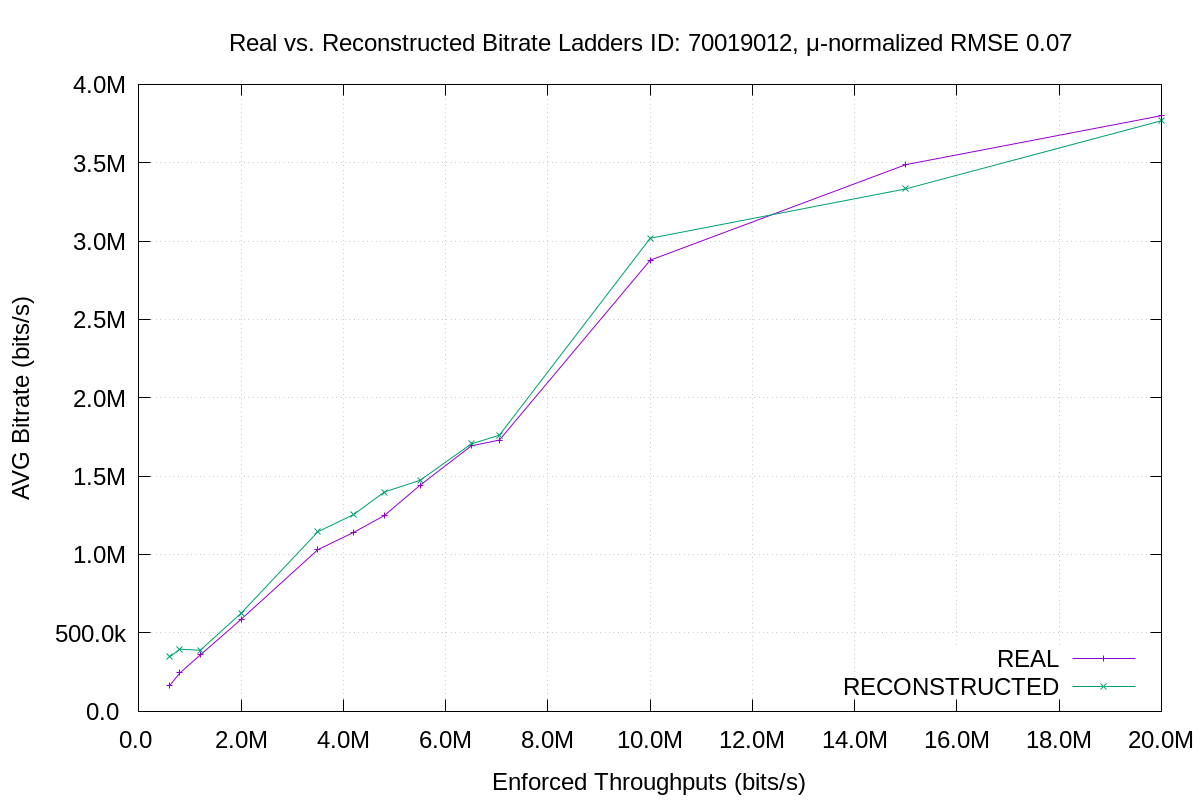
\includegraphics[width=\columnwidth]{img/70019012.png}
  \caption{Comparison between the HAR-based bitrate ladder (REAL) and the
  ADU-based reconstructed bitrate ladder for "Casino" ID: 70019012. Accuracy of
  reconstruction is shown as the RMSE.}
  \label{fig:bl_comparison_good}
\end{figure}

The plot above represents the "real" and reconstructed bitrate ladders.  The
accuracy of our prediction is represented by the RMSE, which is 0.07.  This
title's bitrate ladder gets reconstructed faithfully, and almost every title in
our database follow this trend. This is confirmed by further looking at the
average RMSE shown at the end of \Cref{tab:bitrate_ladders_stats}. Eventually,
63 titles have an RMSE less than 0.12, and 87 less than 0.16.
\Cref{fig:bl_comparison_good_1} and \Cref{fig:bl_comparison_good_2} are two
examples of reconstruction which RMSE is 0.12 and 0.16 respectively.

\newpage

\begin{figure}[!h]
  \centering
  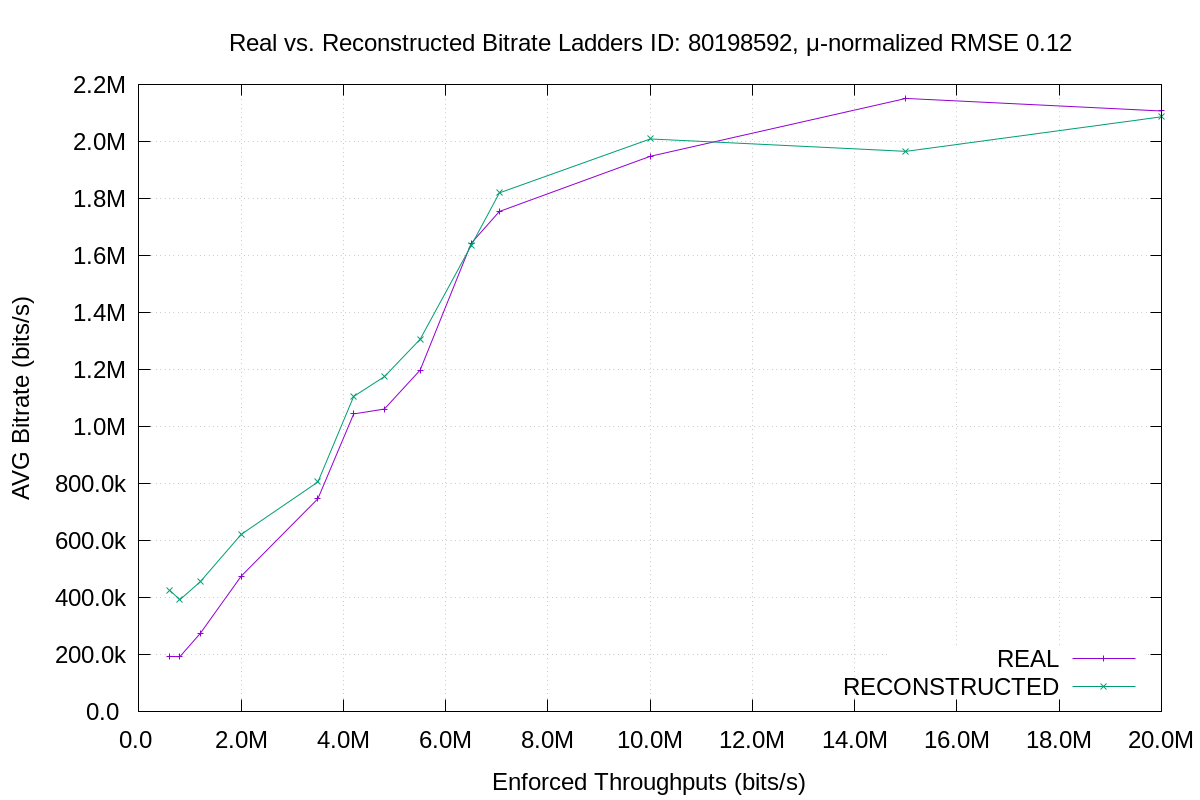
\includegraphics[width=\columnwidth]{img/80198592}
  \caption{Comparison between the HAR-based bitrate ladder (REAL) and the
  ADU-based reconstructed bitrate ladder for "Armed Response" ID: 80198592.
  Accuracy of reconstruction is shown as the RMSE.}
  \label{fig:bl_comparison_good_1}
\end{figure}

By looking at the above plot we spot two major areas where the differences
between the real and the reconstructed bitrates have greater impact on the
overall accuracy. Bottom left, when the enforced bandwidth and the bitrates are
low, and top right, at 15\emph{Mbps}. We focus our attention on the bottom-left
area, and notice how it correlates with the RMSE of the following plots.

\newpage
\begin{figure}[!h]
  \centering
  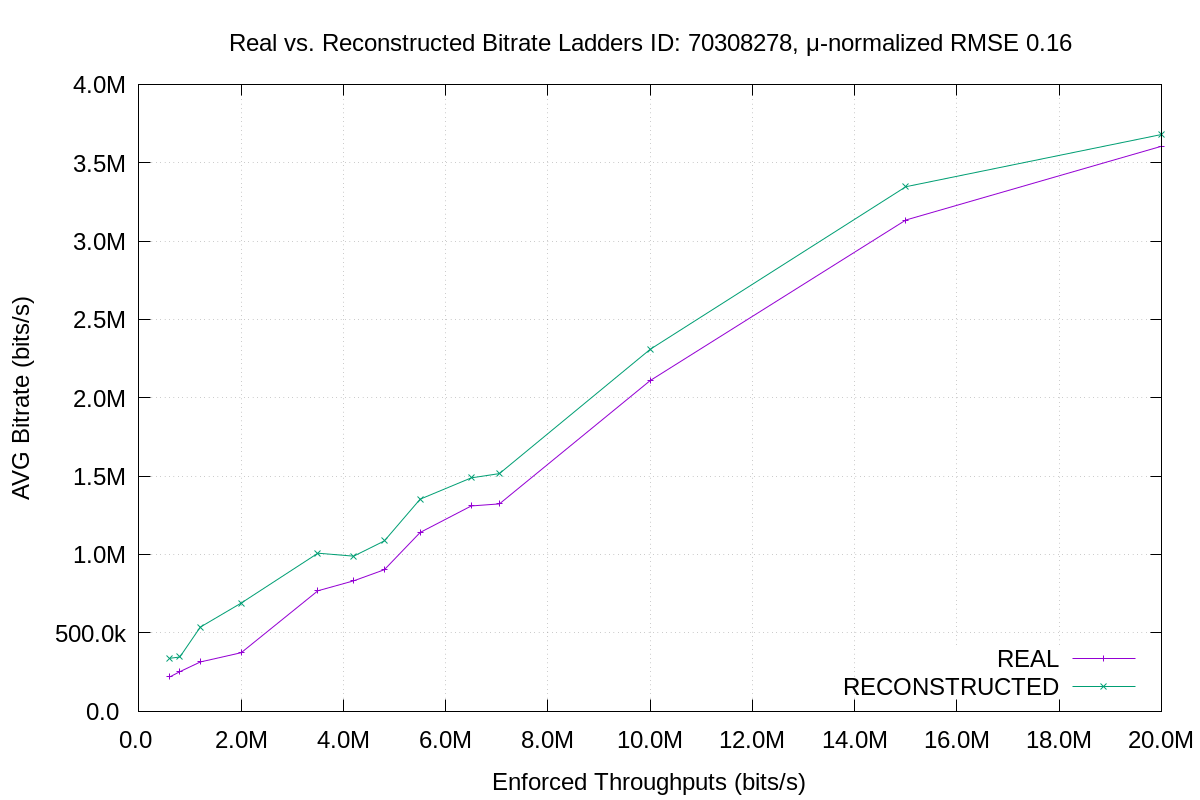
\includegraphics[width=\columnwidth]{img/70308278}
  \caption{Comparison between the HAR-based bitrate ladder (REAL) and the
  ADU-based reconstructed bitrate ladder for "Mission Blue" ID: 80198592.}
  \label{fig:bl_comparison_good_2}
\end{figure}

In this case we observe that with a greater RMSE, the two curves start to be
parallel to each other. By looking at the plot in \Cref{fig:bl_comparison_bad}
we see a magnified version of this behavior, and explain its existence.

\begin{figure}[!h]
  \centering
  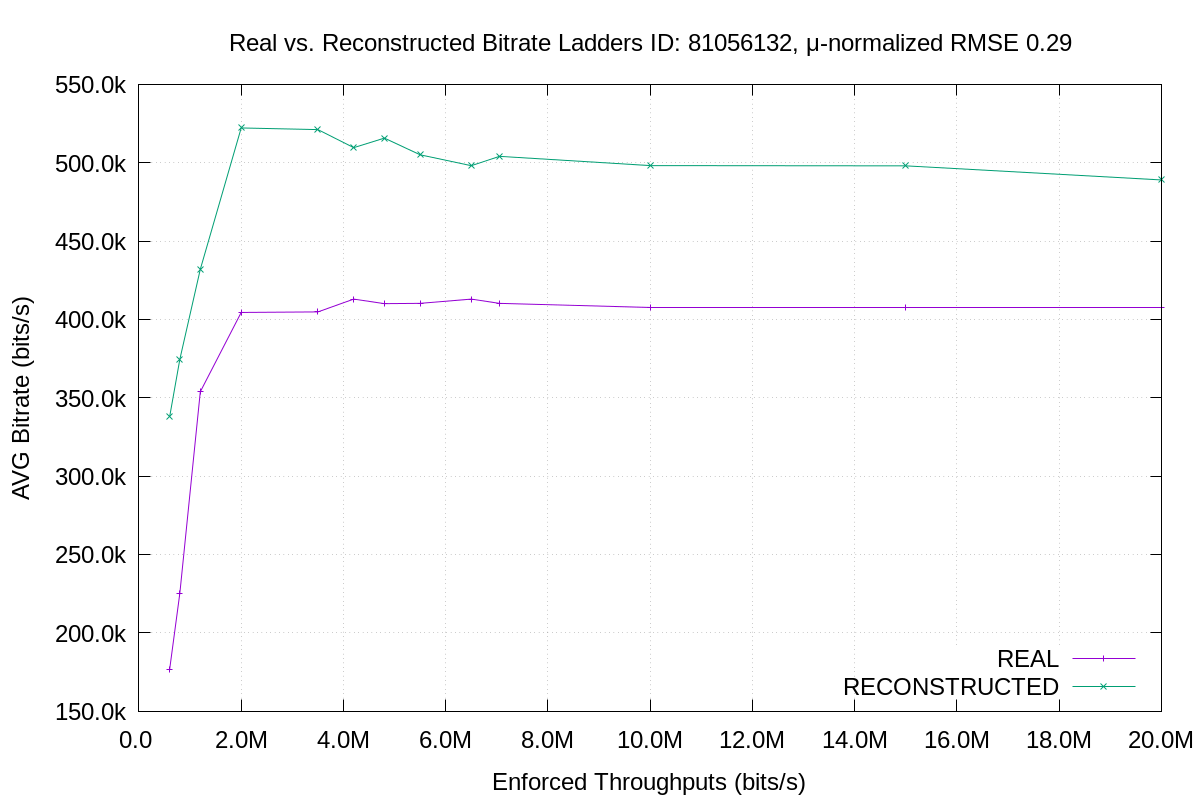
\includegraphics[width=\columnwidth]{img/81056132.png}
  \caption{Comparison between the HAR-based bitrate ladder (REAL) and the
  ADU-based reconstructed bitrate ladder for "Dirty John" ID: 81056132.}
  \label{fig:bl_comparison_bad}
\end{figure}

This plot represent a particular case of a

\todo{Finish this by explaining uniqueness of the bitrate ladders, arguing that
in a bigger DB we should try to cluster and complete the Video Identification
analysis, possibly making comparisons}
